\documentclass[runningheads]{comsis2}

\def\journalissue{Computer Science and Information Systems 0(0):1--6}
\def\paperidnum{DOI: N/A}
\setcounter{page}{1}

\usepackage[dvipdfm]{hyperref}
\usepackage{verbatim}
\usepackage{graphicx}

\title{Authors' Instructions for the Preparation\\of Camera-Ready Contributions with \LaTeX}
\titlerunning{Authors' Instructions}
\author{Vladan Deved\v{z}i\'c\inst{1} \and Marijana Despotovi\'c\inst{1} \and Ivan Lukovi\'c\inst{2} \and
        Violeta Damjanovi\'c\inst{3} \and Milo\v{s} Radovanovi\'c\inst{4}}
\authorrunning{Author(s)}
\institute{Faculty of Organizational Sciences, POB 52\\
  11000 Belgrade, Serbia\\
  \email{\{devedzic,maja\}@fon.rs}
  \and
  Faculty of Technical Sciences, Trg D.\ Obradovi\'ca 6\\
  21000 Novi Sad, Serbia\\
  \email{ivan@uns.ac.rs}
  \and
  Postal Savings Bank, 27.\ marta 71\\
  11000 Belgrade, Serbia\\
  \email{vdamjanovic@posted.co.rs}
  \and
  Dept.\ of Mathematics and Informatics, Trg D.\ Obradovi\'ca 4\\
  21000 Novi Sad, Serbia\\
  \email{radacha@dmi.uns.ac.rs}}

\begin{document}

\maketitle

\begin{abstract}
The abstract should summarize the contents of the paper and should contain at
least 70 and at most 150 words. It should be set using the \texttt{abstract}
environment.

\vspace{6pt}\textbf{Keywords:} computer science, information systems, \LaTeX,
typesetting.
\end{abstract}

\section{Introduction}

These instructions and the corresponding \LaTeX\ style are based
on the corresponding Springer instructions and \LaTeX\ document class for
preparing camera ready papers to be published in the Springer series Lecture
Notes in Computer Science.

The preparation of manuscripts which are to be reproduced by photo-offset
requires special care. Papers submitted in a technically unsuitable form will
be returned for retyping, or canceled if the volume cannot otherwise be
finished on~time.

\section{Manuscript Preparation}

You are encouraged to use \LaTeX\ for the preparation of your camera-ready
manuscript together with the corresponding document class comsis.cls (see
Sect.~\ref{sec:latex}), and send all necessary source files. Please follow
these instructions closely in order to make the volume look as uniform as
possible. Please also send a corresponding pdf file.

We would like to stress that the class/style files should not be manipulated
and that the guidelines regarding font sizes and format should be adhered to.
This is to ensure that the end product is as homogeneous as possible.

\subsection{Printing Area}

The printing area is 125mm $\times$ 197mm. The text should be justified to
occupy the full line width, so that the right margin is not ragged, with words
hyphenated as appropriate. The length of the text on a page should not be less
than~180mm.

\subsection{Layout, Typeface, Font Sizes, and Numbering}

The default font for all text formatting is Times. Use 10-point type for the
name(s) of the author(s) and 9-point type for the address(es) and the abstract.
For the main text, please use 10-point type and single-line spacing. Italic type
may be used to emphasize words in running text. Bold type and underlining should
be avoided. With these sizes, the interline distance should be such that some 45
lines occur on a full-text page.

\subsubsection{Headings.} Headings should be capitalized (i.e., nouns, verbs, and
all other words except articles, prepositions, and conjunctions should be set
with an initial capital) and should, with the exception of the title, be
aligned to the left. Words joined by a hyphen are subject to a special rule.
If the first word can stand alone, the second word should be capitalized.
Headings and appropriate \LaTeX\ commands are enumerated in
Table~\ref{tbl:headings}.

\begin{table}
\caption{Font sizes of headings. Table captions should always be positioned
\emph{above} the tables. Tables should be horizontally centered. The final
sentence of a table caption should end without a period}\label{tbl:headings}
\centering
\setlength\tabcolsep{0.5em}
\begin{tabular}{lll}
\hline
Heading level      & Example                                    & \LaTeX\ command \\ \hline \\[-2ex]
Title (centered)   & \textbf{\Large Authors' Instructions\dots} & \texttt{$\backslash$title} \\
1st-level heading  & \textbf{\large 1.\ Introduction}           & \texttt{$\backslash$section} \\
2nd-level heading  & \textbf{2.1.\ Printing Area}               & \texttt{$\backslash$subsection} \\
3rd-level heading  & \textbf{Headings.} Text follows\dots       & \texttt{$\backslash$subsubsection} \\
4th-level heading  & \textit{Remark.} Text follows\dots         & \texttt{$\backslash$paragraph} \\ \hline
\end{tabular}
\end{table}

Here are some examples of headings: ``Criteria to Disprove Context-Freeness of
Collage Languages'', ``On Correcting the Intrusion of Tracing
Non-deterministic Programs by Software'', ``A User-Friendly and Extendable
Data Distribution System'', ``Multi-flip Networks: Parallelizing GenSAT'',
``Self-determinations of Man''.

\subsubsection{Lemmas, Propositions, and Theorems.} The numbers accorded to lemmas,
propositions, and theorems etc.\ should appear in consecutive order, starting
with the number 1, and not, for example, with the number 11.

\subsection{Figures and Photographs}

Please produce your figures electronically, if possible, and refer to them
from your source file using, for example, the
\texttt{$\backslash$includegraphics} command from package \texttt{graphicx}.
Format the figures using the standard \texttt{figure} environment, and center
them horizontally.

Check that in line drawings, lines are not interrupted and have constant
width. Grids and details within the figures must be clearly readable and may
not be written one on top of the other. Line drawings should have a resolution
of at least 800dpi (preferably 1200dpi). For digital halftones 300dpi is
usually sufficient. The lettering in figures should have a height of 2mm
(10-point type). Figures should be scaled up or down accordingly. Please do
not use any absolute coordinates in figures. If possible, the files of figures
(e.g.\ eps files) should not contain binary data, but be saved in ASCII
format.

Figures should be numbered and should have a caption which should always be
positioned under the figures, in contrast to the caption belonging to a table,
which should always appear above the table. The final sentence of a caption,
be it for a table or a figure, should end without a period. The
\texttt{$\backslash$caption} command will center the captions between the
margins and set them in 9-point type (Fig.~\ref{fig:afigure} shows an
example). The distance between text and figure should be about~8mm, the
distance between figure and caption about~5mm.

\begin{figure}
\centering
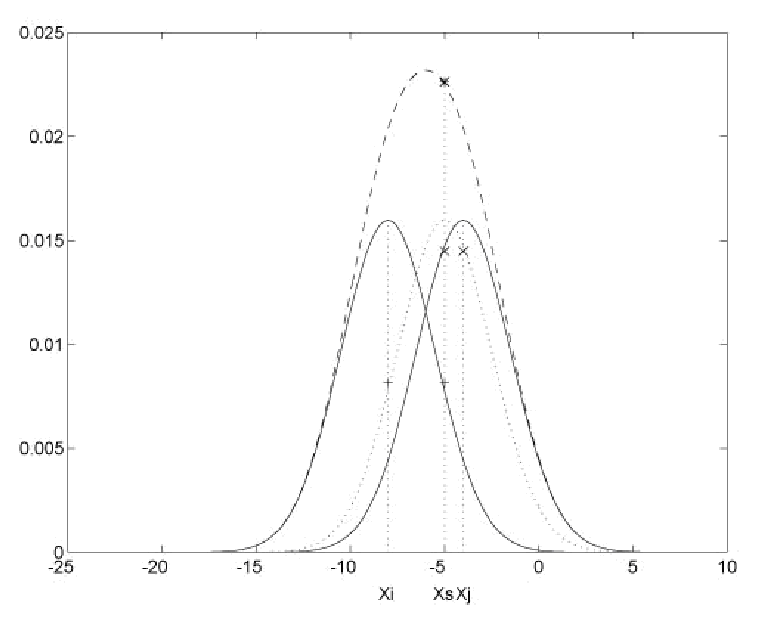
\includegraphics[width=.7\textwidth]{figure}
\caption{One kernel at~$x_s$ (\emph{dotted kernel}) or two kernels at $x_i$ and~$x_j$
(\emph{left and right}) lead to the same summed estimate at~$x_s$. This shows
a figure consisting of different types of lines. Elements of the figure described
in the caption should be set in italics, in parentheses, as shown in this sample
caption. The last sentence of a figure caption should generally end without a period}\label{fig:afigure}
\end{figure}

\paragraph{Remark 1.} In the printed volumes, illustrations are generally black and
white (halftones), and only in exceptional cases, and if the author is
prepared to cover the extra cost for color reproduction, are color pictures
accepted. If color illustrations are necessary, please send us color-separated
files if possible. Color pictures are welcome in the electronic version at no
additional cost.

\paragraph{Remark 2.} To ensure that the reproduction of your illustrations is of
reasonable quality we advise against the use of shading. The contrast should
be as pronounced as possible. This particularly applies for screenshots.

\subsection{Formulas}

Displayed equations or formulas are centered and set on a separate line (with
an extra line or halfline space above and below). Displayed expressions should
be numbered for reference. The numbers should be consecutive within each
section or within the contribution, with numbers enclosed in parentheses and
set on the right margin. For example,
\begin{equation}
x + y = z\,.
\end{equation}

Please punctuate a displayed equation in the same way as ordinary text but
with a small space before the end punctuation.

\subsection{Program Code}

Program listings or program commands in the text are normally set in
typewriter font (Courier).

Example of a Computer Program from Jensen K., Wirth N. (1991) Pascal user
manual and report. Springer, New York:

\begin{verbatim}
  program Inflation (Output)
    {Assuming annual inflation rates of 7%, 8%, and
    10%,...   years};
    const  MaxYears = 10;
    var    Year: 0..MaxYears;
           Factor1, Factor2, Factor3: Real;
    begin
      Year := 0;
      Factor1 := 1.0; Factor2 := 1.0; Factor3 := 1.0;
      WriteLn('Year 7% 8% 10%'); WriteLn;
      repeat
        Year := Year + 1;
        Factor1 := Factor1 * 1.07;
        Factor2 := Factor2 * 1.08;
        Factor3 := Factor3 * 1.10;
        WriteLn(Year:5,Factor1:7:3,Factor2:7:3,
          Factor3:7:3)
      until Year = MaxYears
  end.
\end{verbatim}

\subsection{Footnotes}

The superscript numeral used to refer to a footnote appears in the text either
directly after the word to be discussed or -- in relation to a phrase or a
sentence -- following the punctuation sign (comma, semicolon, or period).
Footnotes are set at the bottom of the normal text area, with a line of
about~5cm immediately above them.\footnote{The footnote numeral is set flush
left and the text follows with the usual word spacing. Second and subsequent
lines are indented. Footnotes should end with a period.}

\subsection{Citations}

The list of references is headed ``References'' and is not assigned a number
in the decimal system of headings. The list should be set in small print and
placed at the end of your contribution, in front of the appendix, if one
exists. Please do not insert a pagebreak before the list of references if the
page is not completely filled. An example is given at the end of this
information sheet. For citations in the text please use the
\texttt{$\backslash$cite} command, and organize your references using Bib\TeX,
with \texttt{$\backslash$bibliographystyle\{splncs03\}}, producing numbered
citations in square brackets, such as: \cite{Agrawal94VLDB}, \cite{Enc97LNCS},
\cite{DatabaseBook02}, \dots

\subsection{Page Numbering and Running Heads}

Page numbers and running heads are automatically generated by \LaTeX. If the
title of your paper is too long for the header please specify a running title
using the \texttt{$\backslash$titlerunning} command. Other parameters will be
allocated by the publisher.

\subsection{Printing Quality}

You are normally not expected to send a printed copy of your manuscript if you
provide the source and pdf files matching exactly each other when printed.
Only in exceptional cases, you will be asked to send sheets which are printed
on one side only. In such a case, please use a high-resolution printer,
preferably a laser printer with at least 300dpi. We prefer the text to be
centered on the pages (i.e., equal margins left and right and top and bottom).
The format of the paper (A4, Letter, etc.) is irrelevant.


\section{Using \LaTeX}\label{sec:latex}

We encourage using \LaTeX\ for preparing final manuscripts. We provide the
document class comsis.cls to help \LaTeX\ users prepare their camera-ready
manuscript and to enable us to use their source files. The necessary style
files and documentation can be downloaded from the ComSIS Web page at
\url{http://www.comsis.org/information.php}.


\section{Supplementary Material}

If you wish to include color illustrations in the electronic version in place
of or in addition to any black and white illustrations in the printed version,
please provide the managing editor and the editorial assistant with the
appropriate files.

If you have supplementary material, e.g., executable files, video clips, or
audio recordings, on your server, simply send the managing editor and the
editorial assistant a short description of the supplementary material and
inform them of the URL at which it can be found. We will add the description
of the supplementary material to the online version of the corresponding
ComSIS volume and create a link to your server. Alternatively, if this
supplementary material is not to be updated at any stage, then it can be sent
directly to the managing editor and the editorial assistant, together with all
the other files.


\section{Copyright Form}

For details regarding the transfer of copyright, please see the ``Copyright
and Use Agreement'' section under ``Information for Contributors'' at the
ComSIS Web page. Generally, we ask contributing authors to complete and sign
the ``Transfer of Copyright'' agreement before the paper may be published. (It
is sufficient if one author from each contribution signs the form on behalf of
all the other authors.) The copyright form is located on our Web page at
\url{http://www.comsis.org/download/ComSISCopyright.doc}. The printed form should be
completed and signed and sent to the editorial assistant by normal mail.
Alternatively, a scanned copy of the form may be sent by e-mail.


\section{Checklist}

When submitting your camera-ready manuscript to the managing editor and the
editorial assistant, please make sure you include the following:
\begin{itemize}
  \item your source (input) files, including the figures;
  \item a single-sided printout (not a photocopy) of the final version of your contribution, if requested by the managing editor;
  \item any style files, templates, and special fonts you may have used;
  \item the completed and signed copyright form.
\end{itemize}

If supplementary material is available, please provide the editorial
assistant~with:
\begin{itemize}
  \item a short description of the supplementary material;
  \item the supplementary material or the URL at which it can be found;
  \item the files of color figures for the electronic version.
\end{itemize}

\nocite{Temporal97TDS,CS95,Ontology02}

\bibliographystyle{splncs03}
\bibliography{example}

\end{document}
